\section{Related Work}
\label{sec:related_work}
\hongyi{Move the stuff about USB protocol to Background}\\
\outline{Attack based on USB 1.0, briefly}\\
\outline{Attack based on USB 2.0, focus on works about application and transport layer}\\
\outline{Attack survey table}\\
\outline{Attack or current works about USB Type-C}\\

In this part, we survey related works on USB attack in Section~\ref{subsec:usb_attack}, and USB defence security in Section \ref{subsec:usb_defence}, respectively.

\subsection{USB Attack}
\label{subsec:usb_attack}
\chaozu{DoS(Fuzzing), Code injection, HID emulation, JFC, our work}
During the development of USB protocol, there are many USB-based attacks were proposed, ranging from DoS (denial of service) to protocol masquerading. Here we will introduce them following an order of their category.\hongyi{What?}

From the kernel perspective, its USB software stack generally expects devices to follow the USB standard and may not consider corner cases of malformed USB packets. Based on this, Facedancer\cite{facedancer} and Syzkaller\cite{syzkaller} uses fuzzing technique to uncover the bugs lying in the kernel drivers. These bugs can cause kernel crash and lead to a DoS situation. Though this poses a great challenge to the availability of a system, this attack still requires physical access to the host and is unable to cause more damage other than DoS.

In the field of USB security, protocol masquerading is also a widely used attack scheme. Due to the lack of authentication in USB protocol, malicious devices can hide their real functionality with re-written firmware\cite{rubber,badusb, rubberducky2020, usbbypassing, iseeyou, usbdriver}. These works rewrite the firmware of a normal-looking flash drive, which allows it to pretend as other devices. When these modified drives are connected to the host, they will be recognized as keyboard or mouse. Then the attacker can execute malicious payloads as they were using the victim's devices. But due to the limitation of USB 2.0\cite{usb20} protocol, these BadUSB attacks are unable to obtain video feedback from the victim as video were not supported until USB 3.0 \cite{usb30}. Though USB 2.0 does not support video transmission, there exists a protocol called MHL(Mobile High-Definition Link) which extends the USB standard and allow video signal to be transmitted through USB interface. JFC\cite{JFC}, short for juicy filming charging is such a work which abuses this standard and exfiltrate video data from victim without permission. But in JFC, this data exfiltration is not combined with BadUSB attacks and MHL is an outdated standard, which limits its capability.

Besides attacking from the protocol perspective, there are works trying to use USB device as a payload delivery means. Duqu\cite{duqu} uses a user-mode rootkit to hide malicious files on the USB storage device and uses a zero-day exploit\cite{zero-day} to execute the malware automatically. There are also works like \cite{brain, stuxnet, conficker,flame} following the same paradigm and performing code-injection attacks. These attacks are much more damaging and flexible comparing to those previous ones, but they requires certain existing flaw like \cite{zero-day} and USB are merely a payload delivery method.

As a data transmission protocol, USB inevitably leaks electromagnetic signals to the environment which may contains sensitive information. Leveraging this physical phenomenon, there are works like \cite{smartphone, poweremi,revealing,su2017usb, usbgpslocator, bates2014leveraging, badusbhub, usbfinger, side, usbdriver} eavesdropping leaked signals and recovering the sensitive data. In a similar fashion, \cite{usbkiller, cable, usbee, turnip} use the RF transmitter to inject signal to cause physical damage to the host machine. Even though the data, including the video data, could be recovered in this way, these attacks for executing malicious code is too difficult to work, and the invisibility is a problem cannot be ignored due to the spacial locality of radio frequency. 

Since USB 3.1 was introduced with USB Type-C in 2013, display port and HDMI connectors have been provided by USB Type-C, transferring of video data can be combined with the other attacks, like protocol masquerading,  protocol corruption and code injection. This has paved the path for our \tool.




\chaozu{attack table}\\
\chaozu{enum diagram}


\subsection{USB Defence Security}
\label{subsec:usb_defence}
There are already many defenses proposed against BadUSB attacks and a comprehensive investigation of previous work.\cite{sok}.

From the hardware perspective, BadUSB attack requires `D-' and `D+' pins which are defined by protocol to transmitting data.
Without these pins, data can't be transferred via USB cable. Based on this fact, USB Condom \cite{Condom} is a hardware solution to block data channel by adding blocker in the connector. This blocker can cut off the `D-' and `D+' connection while leave power pins intact.
However, this method poses a great challenge to plug-and-play property of USB, as once it is deployed, it will stop all USB functions other than charging. 

Under the premise of ensuring the full functionality of USB devices, there have been some works trying to improve the security during connection establishment.
Windows Defender ATP\cite{windenfenderwhite} maintains a whitelist of USB devices, only devices on the whitelist are allowed to communicate with the host. This prevents all potential attacks from untrusted devices. But this requires users to have a certain safety awareness and technical background to maintain a valid whitelist. For example, a naive user may add the USB device from unknown sources to his/her whitelist without precaution. There are designs can overcome this drawback. For instance, Mohammadmoradi et al\cite{mohammadmoradi2018making} proposes a strategy to generate such a whitelist automatically. This strategy first generates a unique fingerprint for each device based on its functionality. Then these fingerprints are used to maintain a safe and valid whitelist of USB devices. There is another work mediating USB connectivity for Industrial Control. TMSUI\cite{yang2015tmsui} relies on rich experience of administrators to build a whitelist. However, some modified USB devices may hide their real functionality from the user.

To solve this flaw, GoodUSB\cite{tian2015defending} will report the functionality claimed by the device to user and let user decides whether to authorize. When a device is plugged in, GoodUSB will load its driver but limit its functionality until a series of authorizations is completed. These authorizations are designed to be performed manually. As BadUSB is normally unable to obtain the video stream of the host, it is impossible for an attacker to complete these authorization with automatic script. Thus this defense is sufficient for normal BadUSB attack. But if the attacker has the access to victim's screen, GoodUSB will be bypassed easily as the attacker can just complete these authorization manually and perform subsequent attacks.

After the USB enumeration and driver loading, there are also works trying to archive `defense in depth' against BadUSB attack.
Neuner et al.\cite{neuner2018usblock} prevents BadUSB attacks from malicious flash drive by analyzing the temporal characteristics of BadUSB-like attacks. This defense mechanism is effective because the attacker cannot obtain the screen of the host using just BadUSB. In this case, the malicious device can only inject key stoke in a very short time to reduce the risk of being discovered. This defect causes the typing characteristics of BadUSB to be detectable.  Pham et al. \cite{pham2010optimizing} optimizing windows security features. It can block the execution of unsigned files, the installation of unsigned driver carried on portable media. What's more, in GoodUSB, a VM is deployed in host to as a honeypot to detect and stop malicious behavior of USB devices. 

In addition to injection attacks, data theft attack is also one of the focuses of academic community. As mentioned in Section~\ref{subsec:usb_attack}, there exist an attack called JFC (juicy film charging)\cite{JFC} which abuses the MHL standard to steal video stream from the victim. In order to mitigate this issue, Meng et al.\cite{JFC} proposed a statistical model using status like GPU/CPU usage to detect JFC attack.

To summarize, there exists a clear trade-off between the effectiveness and the plug-and-play property. Though hardware disabling solution like USB Condom archives the almost absolute security, the functionality of USB is scarified. Other solutions like GoodUSB or whitelist are either bypassable or insufficient under certain cases. 
Some vendors may sacrifice defensive capabilities to improve usability, which allows attackers to take advantage of.

We summarize the former effort in USB attack and defense in Table~\ref{table:attack_vs_defense}, which illustrates the effectiveness of each defense against various attacks including our \tool.
\newcommand{\circlefull}{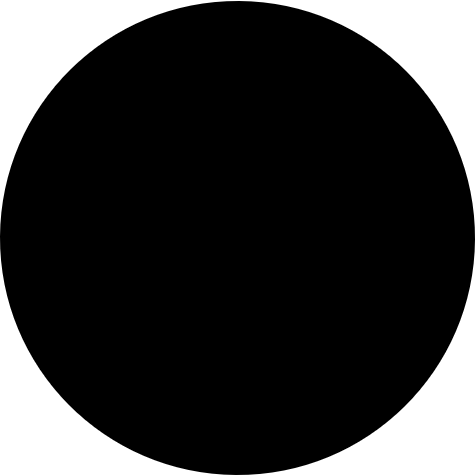
\includegraphics[scale=0.025]{Figs/circle_full.png}}
\newcommand{\circlehalf}{
\includegraphics[scale=0.025]{Figs/circle_half.png}}
\newcommand{\circleempty}{
\includegraphics[scale=0.025]{Figs/circle_empty.png}}
\begin{table*}
	\centering
	\begin{tabular}{|c|c|c|c|c|c|c|c|c|}
		
		\hline
		\diagbox[width=1.46in] {Defence}{Attack} & Facedancer\cite{facedancer}, Syzkaller\cite{syzkaller} & \cite{rubber,badusb, rubberducky2020, usbbypassing, iseeyou, usbdriver} & JFC\cite{JFC}&Duqu\cite{duqu}& \cite{brain, stuxnet, conficker,flame}&\cite{smartphone, poweremi,revealing,su2017usb, usbgpslocator, bates2014leveraging, badusbhub, usbfinger, side, usbdriver} &\cite{usbkiller, cable, usbee, turnip}&Armory\\
		\hline 
		USB condom \cite{Condom}& \circlefull & \circlefull & \circlefull & \circlefull &\circlefull& \circlefull& \circlefull &\circlefull\\
		\hline 
		Windows Defender ATP\cite{windenfenderwhite}, Mohammadmoradi et al\cite{mohammadmoradi2018making}, TMSUI\cite{yang2015tmsui}& \circleempty & \circlehalf & \circlehalf & \circlehalf &\circlehalf& \circleempty& ???????? &\circlehalf\\
		\hline 
		GoodUSB\cite{tian2015defending}& \circlefull & \circlefull & \circlefull & \circlefull &\circlefull& \circleempty& \circlefull &\circleempty\\
		\hline 
		
		Neuner et al.\cite{neuner2018usblock}& \circleempty & \circlefull & \circleempty & \circleempty &\circleempty& \circleempty& \circleempty &\circleempty\\
		\hline 
		Pham et al. \cite{pham2010optimizing}& \circleempty & \circleempty & \circleempty & \circlefull &\circlefull& \circleempty& \circleempty &\circleempty\\
		\hline
		JFCGuard\cite{JFC}& \circleempty & \circleempty & \circlefull & \circleempty &\circleempty& \circleempty& \circleempty & ??? \\
			\hline
	\end{tabular}
	\linebreak
    \begin{tablenotes}
	\footnotesize
	\item[1] \circlefull means that the defense is effective
	\item[2] \circlehalf means that the defense is partial effective
	\item[3] \circleempty means that the defense is uneffective
	\end{tablenotes}
	\caption{Effectiveness of defense against different attacks}
	\label{table:attack_vs_defense}
\end{table*}




